\chapter[Seleção de Características]{Seleção de Características}
\label{ch:caracteristicas}

\section{Aprendizado de Máquina (\textit{Machine Learning})}

A área de Aprendizado de Máquina é considerada um ramo da área de Inteligência Artificial, sendo uma
área especializada no estudo e construção de sistemas que sejam capazes de aprender de
forma automatizada a partir de dados \cite{brink2014}. Desde que os computadores foram inventados, pesquisadores tentam procurar uma maneira de fazer com que eles possam aprender e melhorar sua performance através da experiência. Se fosse possível fazer com que os computadores pudessem aprender, diagnósticos médicos poderiam ser feitos, matérias de jornais que seriam entregues às pessoas de acordo com seus gostos, uma nova maneira de lidar com problemas e situações poderia ser criada \cite{mitchell_1997}.

Por definição, \citeonline{mitchell_1997} diz que um dado programa de computador é capaz de aprender com experiência E, com respeito a um grupo de tarefas T e índice de performance P, se a performance medida por P em T aumenta com E. Ou seja, se conforme o tempo passa, a performance aumenta, ele estará aprendendo.

Existem diversos exemplos de aplicações que aprendem com o tempo e possuem alto grau de acurácia quanto à predição dos possíveis resultados, como por exemplo os sistemas de detecção de spams dos provedores de Email, onde é analisado o texto presente nos emails, o seu email de origem, a frequência desses emails, entre outros dados. No caso de um detector de spam, entende-se pela acurácia do modelo a performance em porcento com que ele consegue classificar corretamente um email, sendo ele spam ou não. O detector de spam utilizaria de uma base de dados de emails para treinar o modelo, sendo essa composto por emails categorizados entre spam e não spam, essa seria a base de dados de treinamento onde ele irá aprender a reconhecer os padrões existentes nos emails, para posteriormente poder predizer e classificar os emails. Temos então que um modelo de Aprendizado de Máquia é composto por um algoritmo de aprendizado de máquina, uma base de dados para realizar o treinamento, e os dados de entrada para serem classficados \cite{mitchell_1997}


\section{Processo de Seleção}

Seleção de Características é um processo que seleciona um subconjunto de um conjunto original de características, a optimicidade do subconjunto é medida por um critéro de avaliação. \cite{liu_2005}. As características são fundamentais para a solução de um dado problema de Aprendizado de Máquina, e quão melhor for essa seleção, melhor será o resultado obtido assim como o tempo necessário para resolve-lo, em termos de acertividade e consumo de recurso computacional. 

As características podem ser de dois tipos: numéricas ou categóricas. As numéricas são representadas por valores, como o próprio nome surgere, já a categórica visa dividir as características em diferentes categorias, não importando a sua ordem. 

O processo de seleção de características geralmente segue quatro passos conforme ilustrado pela Figura 1, sendo eles: geração de subconjuntos (\textit {subset generation}), avaliação do subconjunto (\textit {subset evaluation}), critério de parada (\textit {stopping criterion}), e validação de resultados (\textit {result validation}). De acordo com \citeonline{molina_2002} um subconjunto ideal é aquele que segue uma das seguintes abordagens: a) um subconjuto que possua um tamanho específico que otimize a forma de avaliação. b) um subconjunto de tamanho menor que satisfaça alguma restrição na forma de avaliação. c) o subconjunto com o melhor desempenho levando em consideração sua dimensão e o valor de sua medida de avaliação.

\begin{figure}[h]
	\centering
	\label{fig02}
		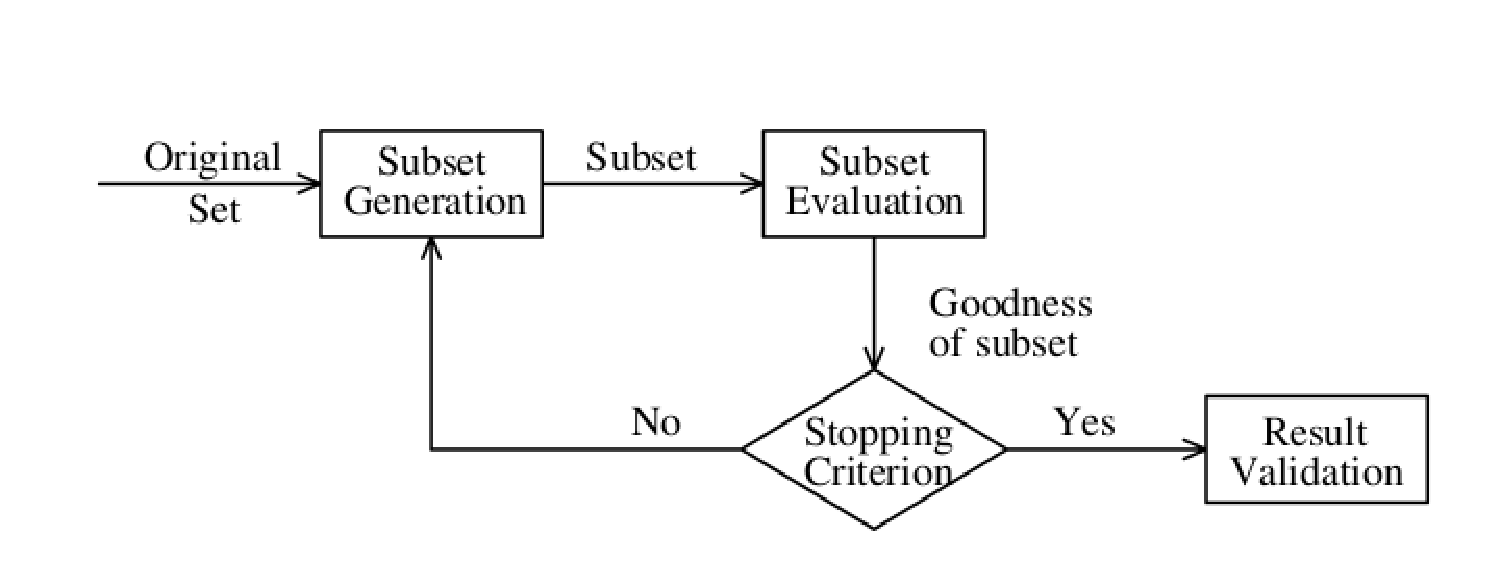
\includegraphics[keepaspectratio=true,scale=0.6]{figuras/fig02.eps}
	\caption{Fluxograma de seleção de características. \cite{liu_2005}}
\end{figure}

\section{Geração de Subconjuntos}

O processo de seleção de características pode ser visto como um problema de busca em que cada um dos estados da busca representa um dos subconjuntos de características \cite{huan_1998}. Imagine um conjunto com três características. Se forem colocadas em um vetor, se posicionariam da seguinte maneira (A1, A2, A3). Tendo em vista que o valor 1 representa a presença da características no subconjunto a ser gerado, temos que em (1, 0, 0) apenas a característica A1 está presente nesse subconjunto. Variando todas as possibilidades partindo de um conjunto com todas as características e chegando a um conjunto com nenhuma. Tal processo está ilustrado na Figura 2.

\begin{figure}[h]
	\centering
	\label{fig03}
		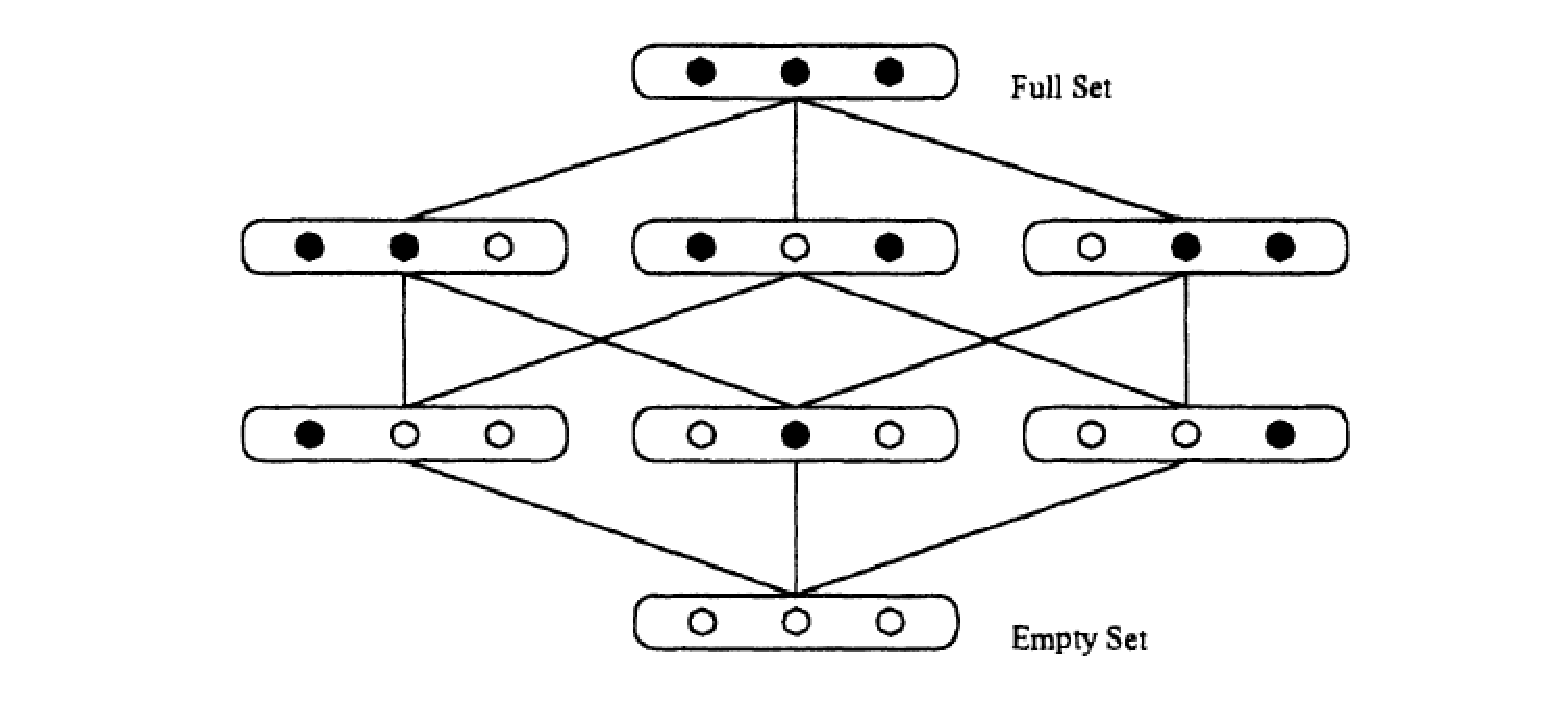
\includegraphics[keepaspectratio=true,scale=0.6]{figuras/fig03.eps}
	\caption{Busca por remoção de características (SBG). \cite{huan_1998}}
\end{figure}

Um dos passos para realizar o processo de seleção de características é escolher a estratégia de busca. A estratégia de busca é a forma como será feito a busca dos subconjuntos a serem avaliados. Existem três maneiras de realizar a busca: busca completa, busca sequencial e busca randomica.

Busca completa - baseia-se em analisar todos os subconjuntos possíveis. Essa busca pode ser exaustiva ou não-exaustiva. A exaustiva buscará analisar todas as combinações, sendo assim, ela se torna um problema da ordem $O(2^N)$. A não-exaustiva busca analisar o máximo de estados possiveis dentro de um determinado limite, buscando evitar comparações desnecessárias para a geração dos subconjuntos \cite{liu_2005}. A busca completa sempre achará o melhor subconjunto, uma vez que ela varre todas as possibilidades, mesmo utilizando técnicas não-exaustivas \cite{dash_1997}.

Busca sequencial - baseia-se em remover ou adicionar características conforme é executado. Esse tipo de busca pode acarretar em perda de alguns subconjuntos ótimos, porém é mais rapido e exige menos recursos computacionais, sendo um problema da ordem de $O(N^2)$. \cite{dash_1997} Existem três formas de realizar esse tipo busca: \textit{sequential forward generation (SFG)}, \textit{ sequential backward generation (SBG)}, \textit{bi-drectional generation}. A primeira consiste em começar com um conjunto vazio e ir adicionando características a ele. Já a \textit{backward} consiste em usar um conjunto completo e ir removendo características sucessivamente. A terceira forma consiste em adicionar e remover simultaneamente, ela é composta por duas buscas simultaneas que geralmente partem do meio do conjunto inicial, com o objetivo de encontrar o melhor subconjunto possível. \cite{liu_2005}. 

Busca randomica - esta segue duas frentes. A primeira utiliza busca sequencial e adiciona as características de forma randomica. A outra frente gera o próximo subconjunto de maneira completamente randomica, ou seja, gera todo o subconjunto de características aleatórias. Tende a ser um problema da ordem de $O(N^2)$ \cite{liu_2005}.

\section{Avaliação do Subconjunto}

\begin{figure}[h]
	\centering
	\label{fig04}
		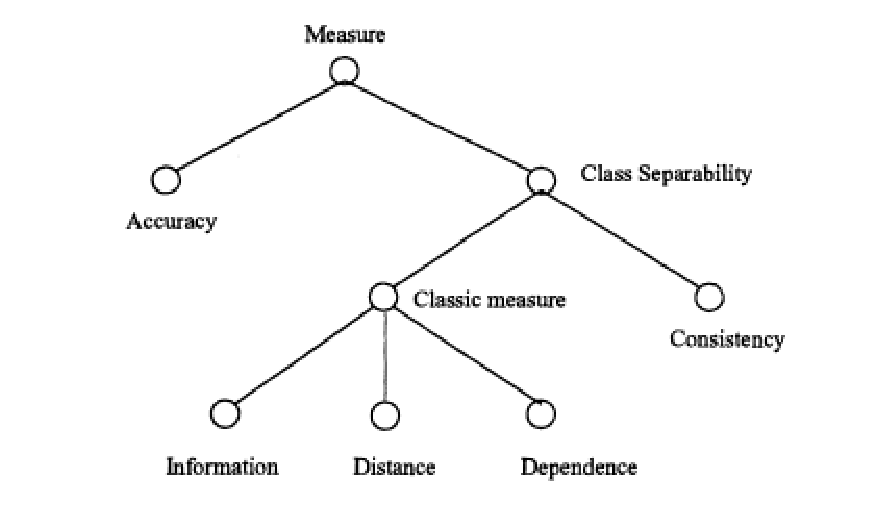
\includegraphics[keepaspectratio=true,scale=1]{figuras/fig04.eps}
	\caption{Hierarquia de Medidas. \cite{huan_1998}}
\end{figure}

Para poder dizer quão bom é um subconjunto é preciso definir um critério. Esses critérios são descritos de acordo com a hierarquia aprsentada na figura 3. As medidas para avaliar uma caracaterística são: medidas de informação (\textit{information measures}), medidas de distancia (\textit{distance measures}), medidas de dependencia (\textit{dependancy measures}), medidas de consistência (\textit{consistency measures}) e medidas de acurácia ({acuracy measures}). \cite{liu_2005, huan_1998} As medidas podem ser divididas em três grupos distintos: a) grupo de medidas classicas, que englobam as medidas de informação, medidas de distancia e medidas de dependencia b) grupo de medidas de consistência, que engloba a própria medida em si c) grupo de medidas de acurácia, que também engloba apenas a medida em si \cite{huan_1998}.

\subsection{Medidas de informação}

A medida de informação determina a informação obtida por uma dada característica \cite{liu_2005}. Isso implica em dizer que uma característica A1 oferece mais informações do que uma característica A2, se dado uma função de incerteza F(x), A1 reduza o grau de incerteza mais do que A2.

\subsection{Medidas de distancia}

Também conhecido como medida de separabilidade, medida de divergencia ou medida discriminativa, essa medida é feita através do calculo da distancia entre duas classes, ou seja, calcular o quanto uma característica consegue  separar duas classes de maneira distinta. Sendo F(X) o calculo da distancia, uma característica A1 separar melhor duas classes do que A2 se F(A1) > F(A2). \cite{huan_1998}

\subsection{Medidas de dependencia}

Conhecida também como medida de correlação ou de similaridade, essa medida visa medir a habilidade de poder predizer o valor de um variável X sabendo o valor de uma variável Y, sendo assim, dado uma função para medir a dependencia F(X, Y), sendo A1 e A2 características distintas, e C a classe, a característica A1 é preferida à característica A2, se F(A1, C) > F(A2, C), ou seja, a característica A1 está melhor associada com a classe C do que A2. \cite{huan_1998, liu_2005}

\subsection{Medidas de consistência}

As medidas anteriores tem o propósito de achar as melhores características que consigam destinguir uma classe de outra. Porém elas não conseguem distinguir características que sejam igualmente boas, ou seja, que apontem para um mesmo resultado e gere redundancia nos subconjuntos. A medida de consistência procura achar um menor número de características que seja tão consistente em seprar as classes quanto ao conjunto inicial. Ou seja, dado uma função de consistência F(X, Y) em relação a classe C, o subconjunto S1 será consistente se F(S1, C) = F(Si, C), sendo S o conjunto inicial \cite{liu_2005}

\subsection{Medidas de acurácia}

Essa já é uma medida que é utilizada dentro do classificador, ou seja, é a medida de performance dele. Para um dado subconjunto de características, quanto mais alta for a acurácia do classificador, melhor será esse subconjunto \cite{huan_1998}.

\section{Critério de Parada}

O critério de parada serve para que, dado um conjunto de características e um algoritmo de seleção de características, ao alcançar um determinado estado de seleção ele diga se o subconjunto gerado está bom ou se ainda precisa ser refinado \cite{dash_1997}. Critérios de parada comumente usados são: a) a busca é finalizada; b) algum valor pré-determinado é alcançado, como por exemplo um número minimo ou máximo de características; c) a adição ou remoçao de características não gera um subconjunto melhor; d) um subconjunto satisfatóriamente bom é encontrado, ou seja, ele cumpre alguns pré-requisitos estabelecidos.

Os critérios de parada são comumente utilizados para que não seja necessário realizar toda a busca, uma vez que o trabalho de exaustão da busca demanda muito tempo e recurso.

\section{Validação de resultados}

Para se avaliar os resultado, primeiramente deve-se ter algum conhecimento sobre os dados que foram submetidos para a seleção de características. Existem vários cálculos que podem ser feitos para que seja posível validar que o processo de seleção realmente resultou em um subconjunto com características que resolva o problema de uma maneira melhor do que o conjunto de características iniciais. Podemos utilizar três dimensões para poder verificar se um método de seleção realmente foi efetivo, são eles: acurácia de predição e o número de características selecionadas \cite{huan_1998}. Além dessas dimensões, devemos levar em consideração alguns fatos dos próprios algorítimos em si, como a velocidade de treinamento do algoritmo e a generalidade das características selecionadas. 

Uma maneira bem comum de se validar os resultados é verificar se a acurácia do classificador foi melhorada, ou se a diminuição do número de características reduziu o tempo de treinamento e execução de um dado classificador sem prejudicar a sua acurácia \cite{liu_2005}.

